\documentclass[models.tex]{subfiles}
\begin{document}
\section{Data Modelling} % (fold)
\label{sec:models}
The first model that was attempted was linear regression, with the hope that it
would produce a strong model for predicting exact values. Since I was willing to
accept merely a `score grade' categorical value rather than the continuous score
rank, decision trees were also investigated.

\subsection{Linear Regression} % (fold)
\label{sub:linear_regression}
With linear regression, it was hoped that all of the numeric values in the
columns would help to create a strong model to predict score rank. The first
step taken was to determine whether or not the tags would prove useful as part
of this venture. In order to investigate, another model was created without the
use of tags to determine how much of a difference their inclusion made.

\begin{figure}[H]
    \centering
    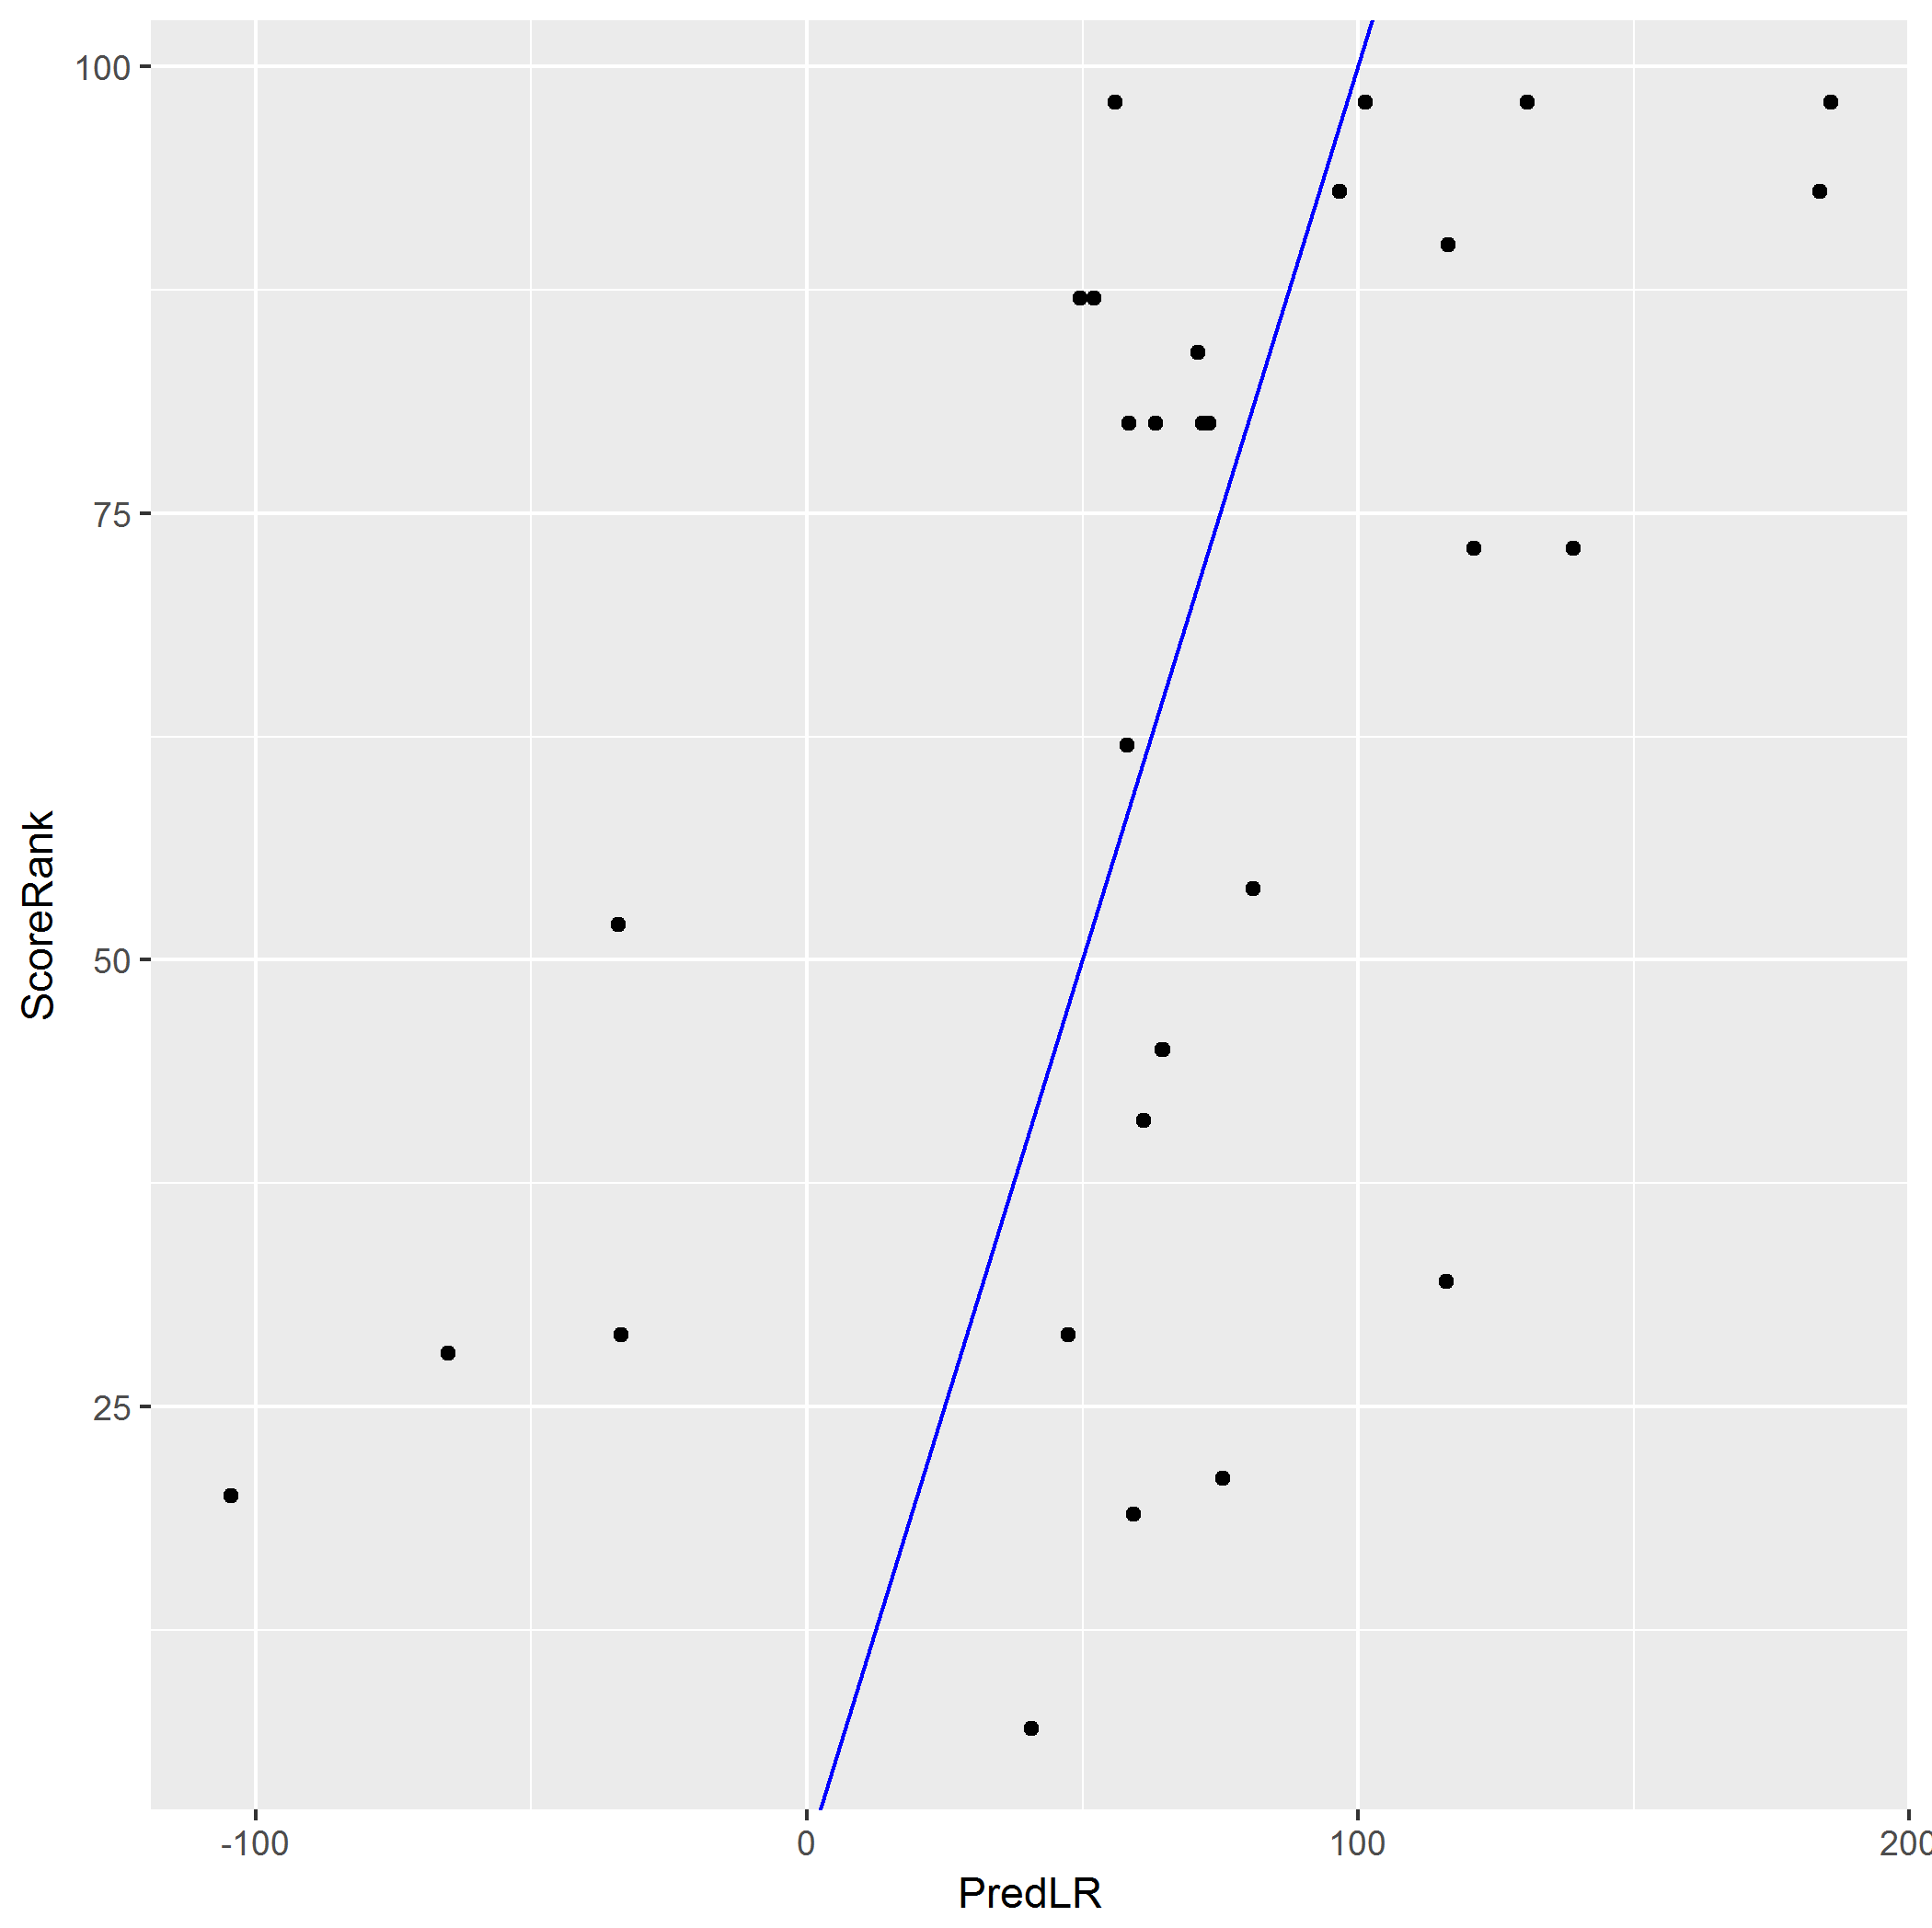
\includegraphics[width=0.45\textwidth]{img/pred.png}
    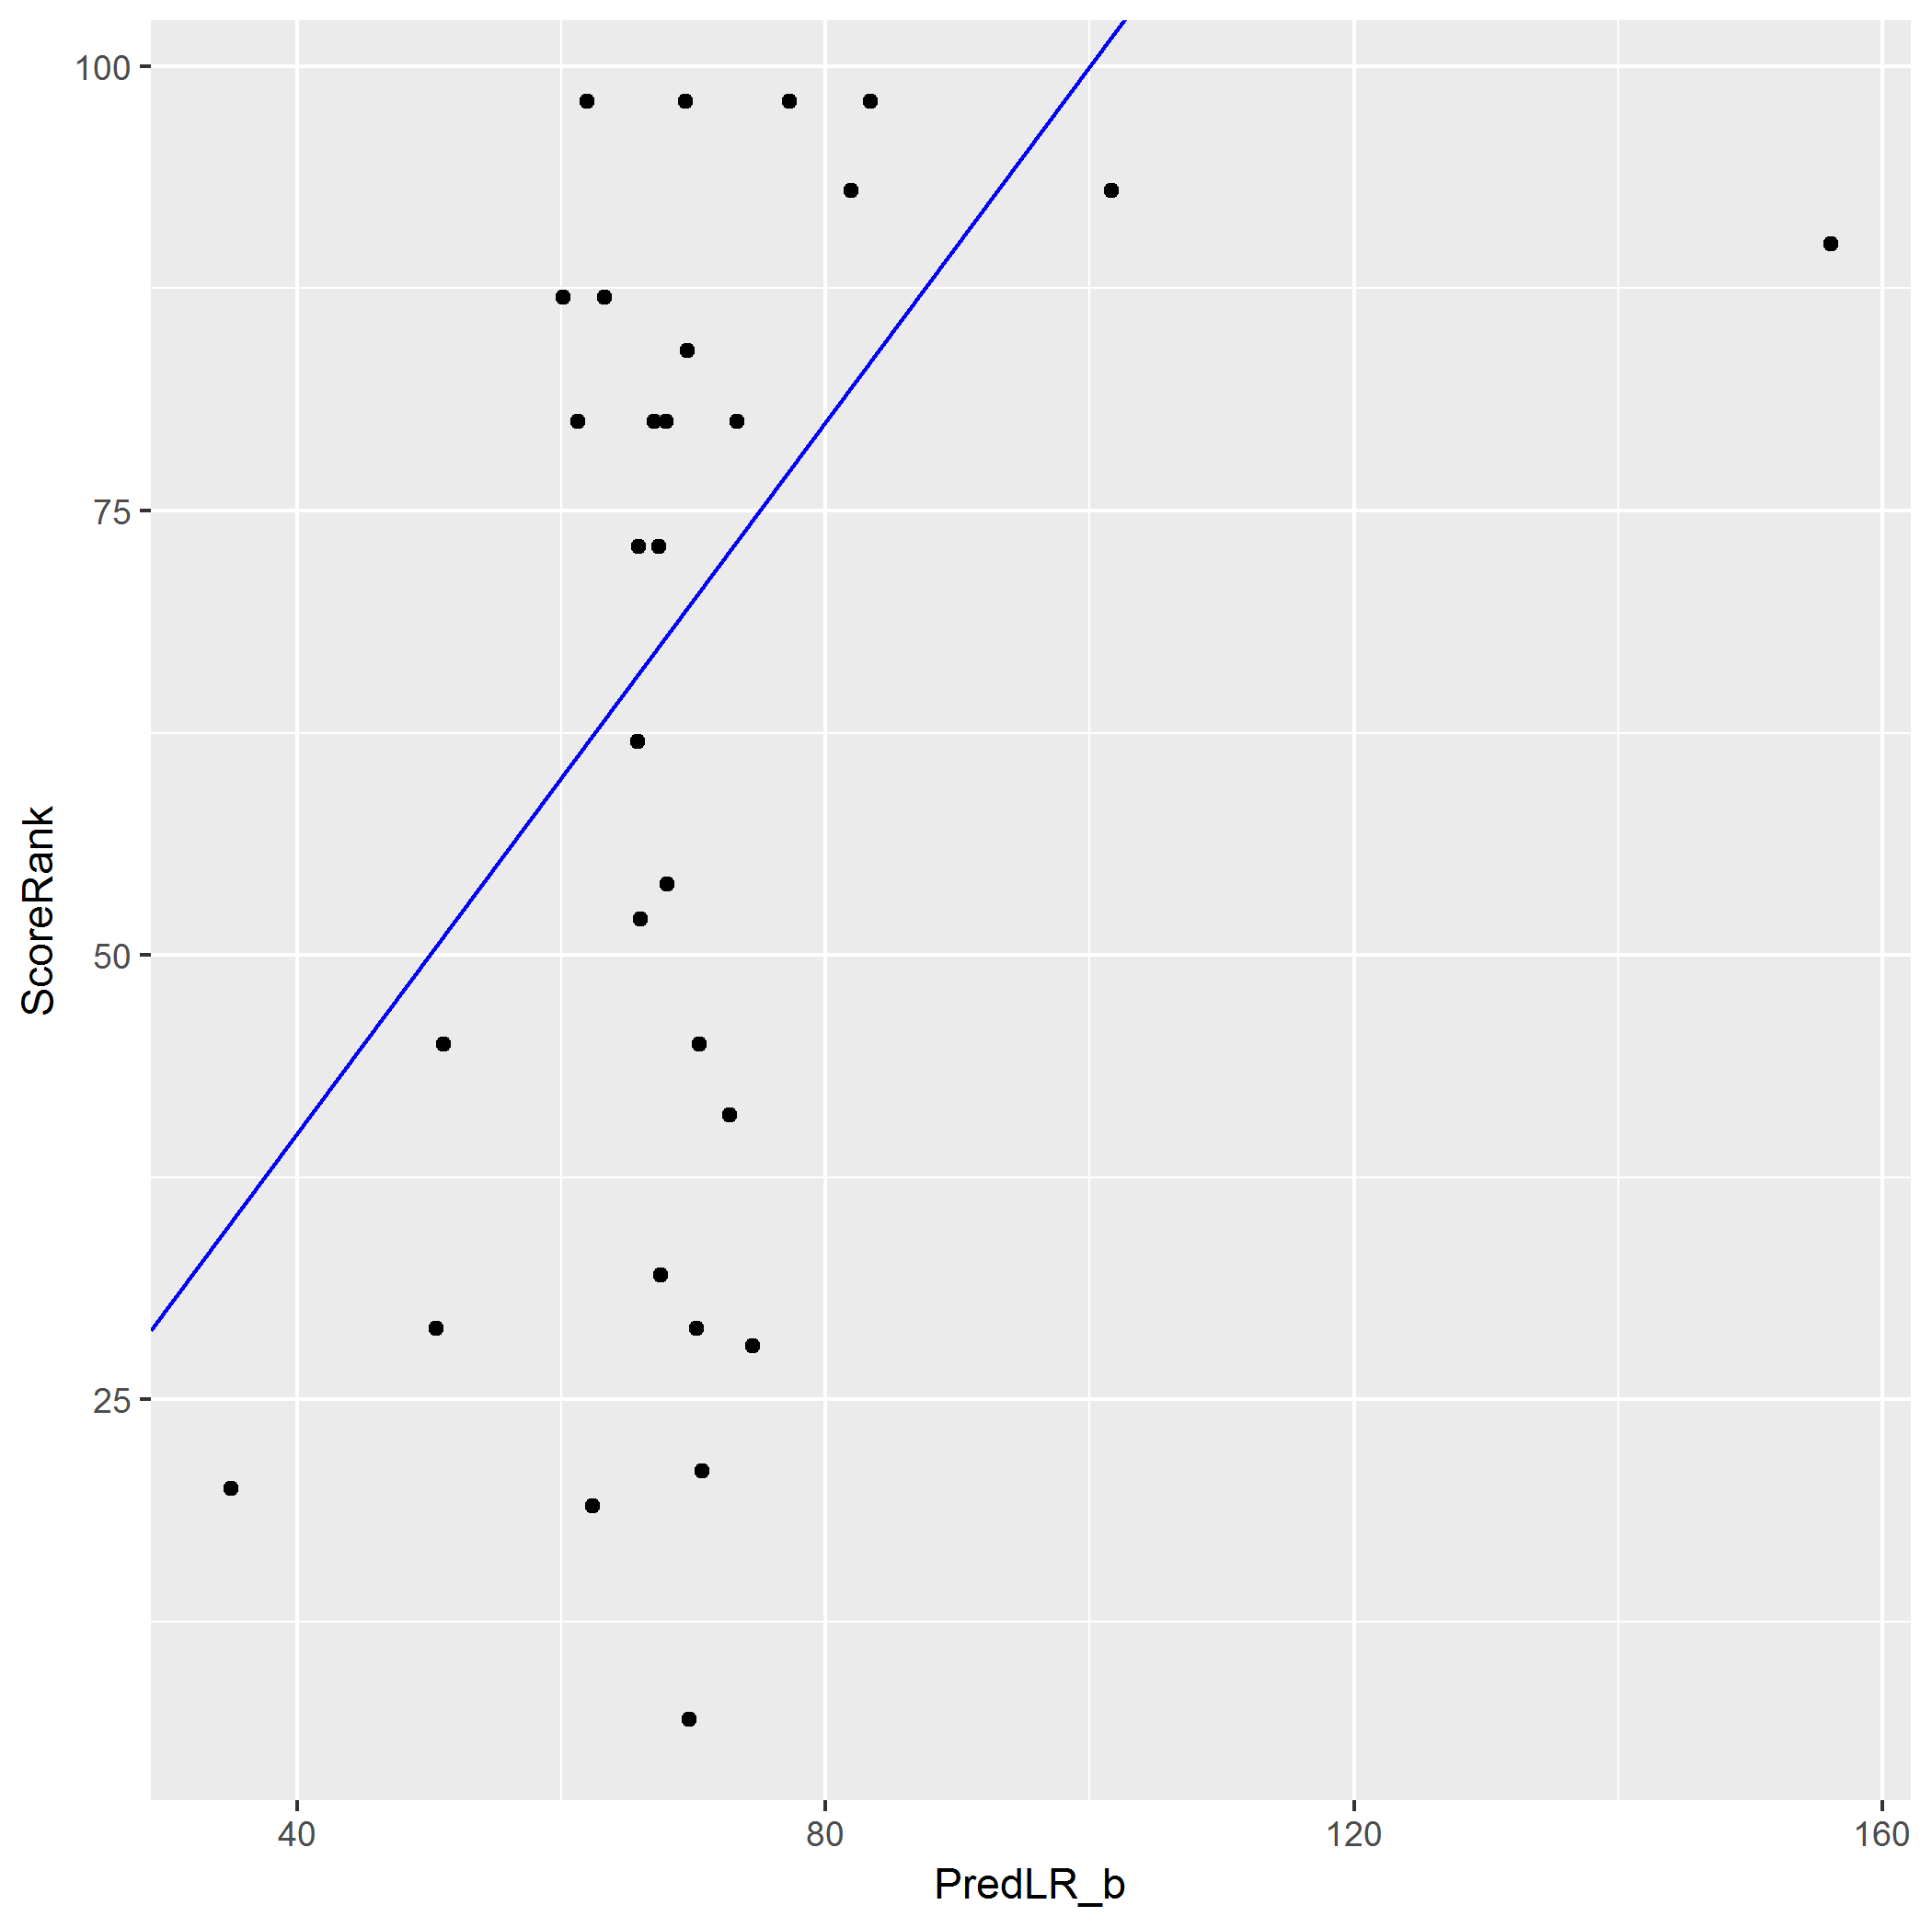
\includegraphics[width=0.45\textwidth]{img/pred_b.png}
    \caption{Linear regression with and without tags}
\end{figure}

The results obtained from these two models are interesting. With tags, the
adjusted R-squared value is 0.4395 while it is 0.1053 when tags are omitted,
which suggests that the inclusion of tags does produce a more accurate model.
However, the RMSE value with tags is 51.7 while it is 29.3 for tags, which
suggests the opposite. This makes it difficult to truly determine which is
better.

The next step was to convert the predicted values into grade, to form a
confusion matrix to further investigate.

\begin{table}[H]
    \centering
    \begin{tabular}{| r | l | l | l | l |}
    \hline
    & \multicolumn{2}{c|}{\textbf{With tags}} &
    \multicolumn{2}{c|}{\textbf{Without tags}} \\
    \hline
    Grade & False & True & False & True \\
    \hline
    0-10 & 1 & 0 & 1 & 0 \\
    10-20 & 1 & 0 & 2 & 0 \\
    20-30 & 2 & 0 & 4 & 0 \\
    30-40 & 0 & 0 & 1 & 0 \\
    40-50 & 3 & 0 & 3 & 0 \\
    50-60 & 1 & 0 & 2 & 0 \\
    60-70 & 1 & 0 & 0 & 1 \\
    70-80 & 2 & 2 & 5 & 1 \\
    80-90 & 3 & 0 & 3 & 0 \\
    90-100 & 1 & 1 & 5 & 0 \\
    \hline
    \end{tabular}
    \caption{Confusion matrix for with and without tags linear regression}
\end{table}

Again, it is clear that linear regression works marginally better when the tags
are included, but it is evident that a strong model cannot be obtained from the
use of linear regression.
% subsection linear_regression (end)

\subsection{Clustering} % (fold)
\label{sub:clustering}

% subsection clustering (end)
% section models (end)
\end{document}